\documentclass{article}
\usepackage{layout}
\usepackage[utf8]{inputenc}
\usepackage[a4paper, total={6in, 8in}]{geometry}
\usepackage{graphicx}
\usepackage{amsmath}


\graphicspath{ {./src/} }

\begin{document}

\section{Question 2A}

% insert graphics here
\begin{center}
    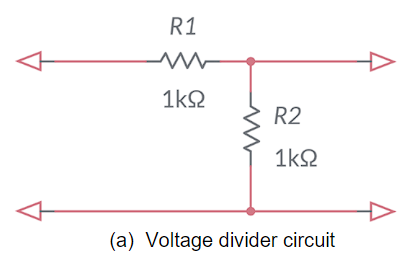
\includegraphics[scale=0.7]{2a.png}

\end{center}

\begin{equation*}
    \begin{aligned}
        V_{out} = \frac{R_2}{R_1 + R_2} V_{in}
    \end{aligned}
\end{equation*}

\begin{equation*}
    \begin{aligned}
        \frac{V_{out}}{V_{in}} = 0.5
    \end{aligned}
\end{equation*}

\begin{equation*}
    \begin{aligned}
        H(s) = 0.5
    \end{aligned}
\end{equation*}

This is a zero order and static system

\section{Question 2B}
\begin{center}
    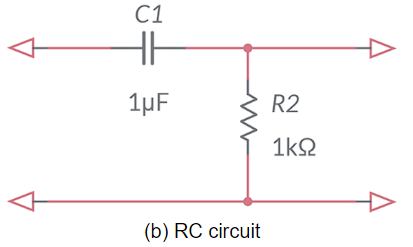
\includegraphics[scale=0.7]{2b.png}

\end{center}


Converting to laplase domain
$
    C_1 = \frac{1}{sC}
$

\begin{equation*}
    \begin{aligned}
        \frac{V_{out}}{V_{in}} = \frac{R_2}{\frac{1}{sC} + R_2}
    \end{aligned}
\end{equation*}

\begin{equation*}
    \begin{aligned}
        \frac{V_{out}}{V_{in}} = \frac{R_2 sC}{1 + R_2 sC}
    \end{aligned}
\end{equation*}

\begin{equation*}
    \begin{aligned}
        H(S) = \frac{s}{s + 10^3}
    \end{aligned}
\end{equation*}

This is a first order and dynamic system


\section{Question 2C}
\begin{center}
    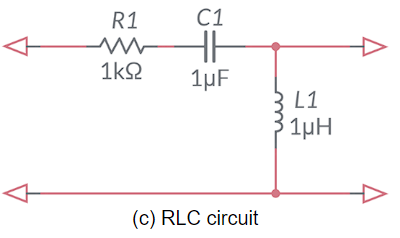
\includegraphics[scale=0.7]{2c.png}

\end{center}

converting to laplase domain
$
    C_1 = \frac{1}{sC}, L_1 = sL
$.

\begin{equation*}
    \begin{aligned}
        \frac{V_{out}}{V_{in}} = \frac{sL}{R_1 + \frac{1}{sC} + sL}
    \end{aligned}
\end{equation*}

\begin{equation*}
    \begin{aligned}
        \frac{V_{out}}{V_{in}} = \frac{s^2LC}{s^2LC + sR_1C + 1}
    \end{aligned}
\end{equation*}

\begin{equation*}
    \begin{aligned}
        H(S) = \frac{s^2 LC}{s^2LC + sR_1C + 1}
    \end{aligned}
\end{equation*}

\begin{equation*}
    \begin{aligned}
        H(S) = \frac{s^2 10^{-12}}{s^2 10^{-12} + s10^{-3} + 1}
    \end{aligned}
\end{equation*}

\begin{equation*}
    \begin{aligned}
        H(S) = \frac{s^2}{s^2 + s10^{9} + 10^{12}}
    \end{aligned}
\end{equation*}

This is a second order and dynamic system


\section{Question 2D}
\begin{center}
    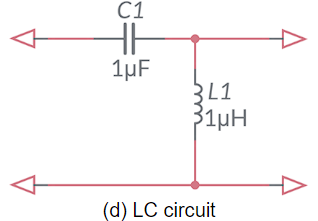
\includegraphics[scale=0.7]{2d.png}

\end{center}

converting to laplase domain
$
    C_1 = \frac{1}{sC}, L_1 = sL
$.

\begin{equation*}
    \begin{aligned}
        \frac{V_{out}}{V_{in}} = \frac{sL}{\frac{1}{sC} + sL}
    \end{aligned}
\end{equation*}

\begin{equation*}
    \begin{aligned}
        \frac{V_{out}}{V_{in}} = \frac{s^2LC}{s^2LC + 1}
    \end{aligned}
\end{equation*}

\begin{equation*}
    \begin{aligned}
        H(S) = \frac{s^2LC}{s^2LC + 1}
    \end{aligned}
\end{equation*}

\begin{equation*}
    \begin{aligned}
        H(S) = \frac{s^2 10^{-12}}{s^2 10^{-12} + 1}
    \end{aligned}
\end{equation*}

\begin{equation*}
    \begin{aligned}
        H(S) = \frac{s^2}{s^2 + 10^{12}}
    \end{aligned}
\end{equation*}
This is a second order and dynamic system



\end{document}
